%!TEX root = ../main.tex
%%%%%%%%%%%%%%%%%%%%%%%%%%%%%%%%%%%%%%%%%%%
%
%LEZIONE 29/02/2016 - SECONDA SETTIMANA (1)
%
%%%%%%%%%%%%%%%%%%%%%%%%%%%%%%%%%%%%%%%%%%%
\chapter{Varietà topologiche}
%%%%%%%%%%%%%%
%INTRODUZIONE%
%%%%%%%%%%%%%%
\section{Introduzione}

\begin{defn}{Sottoinsieme complementare}{complementare}\index{Complementare}
	Sia \(B\) un sottoinsieme dello spazio topologico \(X\).
	Si definisce complementare di \(B\) la differenza insiemistica fra \(X\) e \(B\), ovvero
	\[
		\setc{B}=X\setminus B.
	\]
\end{defn}

\begin{defn}{Insieme chiuso}{chiuso}\index{Insieme!chiuso}
	Un sottoinsieme \(C\) su uno spazio topologico \(X\) si definisce \emph{chiuso} se \(\setc{C}\) è un aperto.
\end{defn}

\begin{oss}
	Si può quindi definire una topologia a partire dai sottoinsiemi chiusi.
\end{oss}

\begin{oss}
	Per definizione \(\emptyset\) e \(X\) sono insiemi chiusi.
\end{oss}

\begin{oss}
	Dire che un insieme è chiuso è diverso da dire che è non aperto, ad esempio, in \(\R^2\), l'insieme rappresentato nella figura \ref{fig:fig1}, non è nè chiuso nè aperto.
\end{oss}

\begin{figure}[tp]
	\begin{centering}
		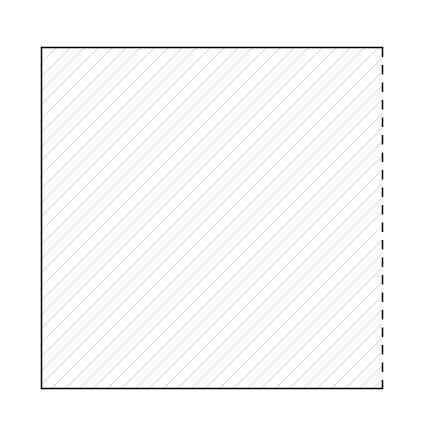
\includegraphics{fig1.png}
		\caption{L'insieme contiene solo tre lati del quadrato}
		\label{fig:fig1}
	\end{centering}
\end{figure}

\begin{prop}{Unione finita di chiusi}{unioneChiusi}
	Unione finita di chiusi è un insieme chiuso.
\end{prop}

\begin{proof}
	Siano \(C_1,\dots,C_n\) sottoinsiemi chiusi di \(X\), dobbiamo dimostrare che il complementare dell'unione è un aperto:
	\[
		\setc{\left(\bigcup_{i=1}^n C_i\right)}=\bigcap_{i=1}^n\setc{C_i},
	\]
	che è aperto in quanto per le proprietà dello spazio topologico.
\end{proof}

\begin{prop}{Intersezione qualsiasi di chiusi}{intersezioneChiusi}
	Intersezione qualsiasi di chiusi è un insieme chiuso.
\end{prop}

\begin{proof}
	Analoga alla precedente.
\end{proof}
%%%%%%%%%%%%%%%%%%%%%%%%%%%%%%%%%%%%%%%%%%%
%
%LEZIONE 02/03/2016 - SECONDA SETTIMANA (2)
%
%%%%%%%%%%%%%%%%%%%%%%%%%%%%%%%%%%%%%%%%%%%
\begin{ese}
	Su \(\R\) con la topologia euclidea, gli intervalli \([a,b],[a,+\infty)\) e \((-\infty,b]\), sono insiemi chiusi.
\end{ese}

\begin{ese}
	In uno spazio metrico \((X,d)\), i dischi chiusi
	\[
		\overline{D_r(x)}=\Set{d(y,x)\le r},
	\]
	sono insiemi chiusi.
\end{ese}

\begin{ese}
	Ogni sottoinsieme è chiuso in un insieme con la topologia discreta.
\end{ese}

\begin{defn}{Applicazione chiusa}{applChiusa}\index{Applicazione!chiusa}
	Un'applicazione \(f\colon X\to Y\) tra spazi topologici si dice \emph{chiusa} se manda chiusi in chiusi, ovvero
	\[
		\setc{f(A)}\in \Tau_Y,\,\fa \setc{A}\in \Tau_X.
	\]
\end{defn}

\begin{oss}
	Un'applicazione \(f\colon X\to Y\) tra spazi topologici è continua se e soltanto se la controimmagine di un chiuso è un chiuso
\end{oss}

\begin{oss}
	Un'applicazione \(f\colon X\to Y\) tra spazi topologici, continua e biiettiva, è un omeomorfismo, se e soltanto se \(f\) è chiusa.
\end{oss}
%%%%%%%%%%%%%%%%%%%%%%%%%%%%%%
%INTERIORI, ESTERIORI E BORDI%
%%%%%%%%%%%%%%%%%%%%%%%%%%%%%%
\section{Interiori, esteriori e bordi}
Con \(X\) faremo sempre riferimento ad un insieme dotato di una topologia \(T\)

\begin{defn}{Chiusura di un insieme}{chiusura}\index{Chiusura}
	Sia \(B\) un sottoinsieme qualsiasi di \(X\).
	Si definisce \emph{chiusura} di \(B\), l'intersezione di tutti i chiusi che contengono \(X\), ovvero
	\[
		\overline{B}=\bigcap\Set{C\subset X | B\subset C\text,C\text{chiuso}}.
	\]
\end{defn}

\begin{oss}
	\(\overline{B}\) è il più piccolo chiuso che contiene \(B\).
\end{oss}

\begin{defn}{Interiore di un insieme}{interiore}\index{Interiore}
	Sia \(B\) un sottoinsieme qualsiasi di \(B\).
	Si definisce \emph{interiore} di \(B\), l'insieme di tutti gli aperti contenuti in \(B\), ovvero
	\[
		\mathring{B}=\bigcup\Set{A\subset X | A\subset B,A\text{ aperto}}.
	\]
\end{defn}

\begin{oss}
	\(\mathring{B}\) è il più grande aperto contenuto in \(B\).
\end{oss}

\begin{oss}
	In generale vale
	\[
		\mathring{B}\subseteq B\subseteq \overline{B},
	\]
	dove l'uguaglianza vale se \(B\) è aperto nel primo caso e se \(B\) è chiuso nel secondo.
\end{oss}

\begin{defn}{Esteriore di un insieme}{esteriore}\index{Esteriore}
	Sia \(B\) un sottoinsieme qualsiasi di \(B\).
	Si definisce \emph{esteriore} di \(B\) il complementare della sua chiusura, ovvero
	\[
		\ext B=\setc{\overline{B}}=X\setminus \overline{B}.
	\]
\end{defn}

\begin{oss}
	Per definizione, l'esteriore di un insieme è sempre aperto.
\end{oss}

\begin{defn}{Bordo di un insieme}{bordo}\index{Bordo}
	Sia \(B\) un sottoinsieme qualsiasi di \(B\).
	Si definisce \emph{bordo} di \(B\) il complementare dell'unione digiunta dell'interiore e dell'esteriore di \(B\), ovvero
	\[
		\pd B=\setc{\{\mathring{B}\sqcup \ext B\}}=X\setminus\{\mathring{B}\cup\ext B\}.
	\]
\end{defn}

\begin{oss}
	Dal momento che l'interiore e l'eseteriore di \(B\) sono entrambi aperti, si avrà che \(\pd B\) è chiuso.
\end{oss}

\begin{oss}
	La figura \ref{fig:fig2} mostra un esempio di sottoinsieme di \(\R^2\) e la sua suddivisione.
\end{oss}

\begin{figure}[tp]
	\begin{centering}
		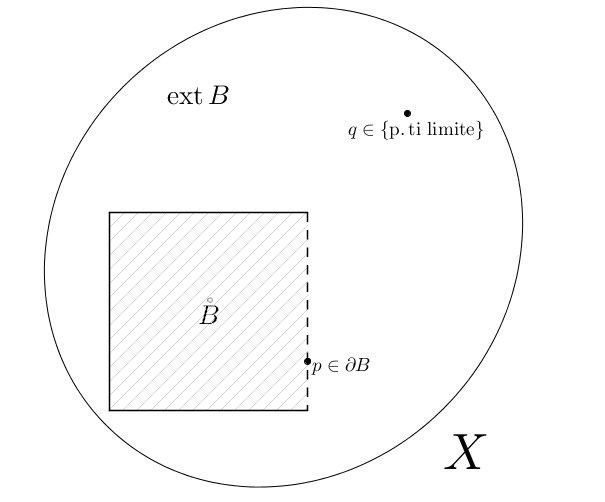
\includegraphics{fig2.png}
		\caption{Un generico insieme in \(\R^2\).}
		\label{fig:fig2}
	\end{centering}
\end{figure}

\begin{lem}\label{lem:intEst1}
	Sia \(B\) un sottoinsieme di \(X\), allora
	\[
		X=\mathring{B}\sqcup \pd B\sqcup \ext B.
	\]
\end{lem}

\begin{proof}
	Segue immediatamente dalla definizione di \(\pd B\).
\end{proof}

\begin{lem}\label{lem:intEst2}
	Sia \(B\) un sottoinsieme di \(X\), allora
	\[
		p\in \mathring{B} \iff \ex U_p\in T:U_p\subseteq B.
	\]
\end{lem}

\begin{proof}
	Dal momento che \(\mathring{B}\) è definito come l'unione degli aperti contenuti in \(B\) si ottiene facilmente la tesi.
\end{proof}

\begin{lem}\label{lem:intEst3}
	Sia \(B\) un sottoinsieme di \(X\), allora
	\[
		p\in \ext B\iff \ex U_p\in T:U_p\cap B=\emptyset.
	\]
\end{lem}

\begin{proof}
	Dal momento che \(\ext B\) è definito come il complementare della chiusura di \(B\), avremo che, se \(p\in \ext B\),
	\[
		\begin{split}
			p\in \setc{\overline{B}} & \iff p\in \setc{\left(\bigcap_{\substack{C\text{ chiuso}\\C\supset B}}C\right)}\\
			& \iff p\in \bigcup_{\substack{C\text{ chiuso}\\C\supset B}}\setc{C}\\
			& \iff p\in \setc{C},
		\end{split}
	\]
	dove \(C\) è chiuso e contiene \(B\), che implica \(\setc{C}\) è aperto e disgiunto da \(B\).
	Quindi
	\[
		p\in \setc{C}\in T,\setc{C}\cap B=\emptyset.
	\]
	Il viceversa si mostra in modo analogo.
\end{proof}

\begin{lem}\label{lem:intEst4}
	Sia \(B\) un sottoinsieme di \(X\), allora
	\[
		p\in\pd B \iff \fa U_p\in T\implies U_p\cap B\neq\emptyset,U_p\cap \setc{B}\neq\emptyset.
	\]
\end{lem}

\begin{proof}
	Segue dai due lemmi precedenti.
\end{proof}

\begin{lem}\label{lem:intEst5}
	Sia \(B\) un sottoinsieme di \(X\), allora
	\[
		B\text{ aperto }\iff B=\mathring{B}.
	\]
\end{lem}

\begin{proof}
	Segue dal lemma \ref{lem:intEst2}.
\end{proof}

\begin{lem}\label{lem:intEst6}
	Sia \(B\) un sottoinsieme di \(X\), allora
	\[
		B\text{ chiuso }\iff B=\overline{B}\iff\pd B\subset B.
	\]
\end{lem}

\begin{proof}
	La prima implicazione segue banalmente dalla definizione.
	Osserviamo che
	\[
		\pd B=\setc{\{\mathring{B}\cup\ext B\}}=\setc{\mathring{B}}\cap\setc{\ext B},
	\]
	ma \(\ext B=\setc{\overline{B}}\), per cui \(\setc{\ext B}=\overline{B}\).
	Quindi
	\[
		\pd B=\setc{\mathring{B}}\cap \overline{B}=\setc{\mathring{B}}\cap B\subset B,
	\]
	in quanto \(\mathring{B}\subset B\).
	Il viceversa è analogo.
\end{proof}

\begin{defn}{Punto limite}{puntoLimite}\index{Punto limite}
	Sia \(B\) un sottoinsieme qualsiasi di \(X\).
	Un punto \(q\in X\), si dice \emph{punto limite}, o di \emph{accomulazione}, per \(B\), se ogni intorno di \(U_q\) contiene un punto di \(B\) distinto da \(q\).
\end{defn}

\begin{oss}
	In generale, preso un sottoinsieme \(B\subset X\), si ha che il bordo di \(B\) è distinto dall'insieme dei suoi punti limite.
	Infatti, se consideriamo
	\[
		\mathcal{R}=\Set{(x,y)\in\R^2 | 1\le x<3,2\le y\le 4},
	\]
	mostrato sempre in figura \ref{fig:fig1}, ed il punto \(q=(6,7)\), possiamo definire il sottoinsieme
	\[
		B=\mathcal{R}\cup\{q\}.
	\]
	In questo caso avremo che il bordo di \(B\) è costituito dai lati di \(\mathcal{R}\) e il punto \(q\).
	D'altronde, l'insieme dei punti limite di \(B\) sarà la chiusura di \(\mathcal{R}\).
\end{oss}

\begin{ese}
	Prendiamo \(X=\R\).
	Avremo che l'insieme dei punti limite di \(\Z\) è vuoto.
	Mentre l'insieme dei punti limite di \(\{\frac{1}{n}\}_{n\in\N}\) sarà \(\{0\}\), che non è un elemento dell'insieme.
\end{ese}

\begin{defn}{Sottoinsieme denso}{denso}\index{Sottoinsieme denso}
	Sia \(B\) un sottoinsieme qualsiasi di \(X\).
	\(B\) si dice \emph{denso} in \(X\) se la sua chiusura coincide con \(X\).
\end{defn}

\begin{pr}
	Sia \(B\) un sottoinsieme di \(X\), allora
	\[
		B\subset X\text{ è denso }\iff\fa x \in X\,\ex x_n \in B : x_n \to x.
	\]
\end{pr}

\begin{pr}
	Sia \(B\) un sottoinsieme di \(X\), allora
	\[
		B\subset X\text{ è denso }\iff A\cap B\neq\emptyset,\,\fa A\in T.
	\]
\end{pr}

\begin{ese}
	\(\Q\) è un sottoinsieme denso in \(\R\) con la topologia euclidea.
\end{ese}

\begin{ese}
	\(\Q^n\) è un sottoinsieme denso in \(\R^n\) con la topologia euclidea.
\end{ese}

\begin{oss}
	Vedremo in seguito che sia \(\Q\) che \(\Q^n\) sono numerabili.
\end{oss}
%%%%%%%%%%%%%%%%%%%%%%
%VARIETA' TOPOLOGICHE%
%%%%%%%%%%%%%%%%%%%%%%
\section{Varietà topologiche}

\begin{defn}{Spazio localmente euclideo}{spazioLocEuclideo}\index{Spazio!localmente euclideo}
	Uno spazio topologico \(X\) si definisce \emph{localmente euclideo} di dimensione \(n\), se ogni punto \(p\in X\), possiede un intorno \(U_p\) tale che \(U_p\) è omeomorfo ad un aperto di \(\R^n\).
\end{defn}

\begin{oss}
	In generale questa definizione implica che ogni intorno \(U_p\) è omeomorfo a tutto \(\R^n\), infatti \(U_p\) è omeomorfo ad un disco \(D_r(x)\) di \(\R^n\), ma
	\[
		D_r(x)\approx D_1(\bar{x})\approx \R^n.
	\]
\end{oss}

\begin{defn}{Spazio di Hausdorff}{spazioHausdorff}\index{Spazio!di Hausdorff}
	Uno spazio topologico \(X\) si dice \emph{di Hausdorff}, o \(T2\), se
	\[
		\fa p,q\in X,\,\ex U_p,U_q:U_p\cap U_q=\emptyset.
	\]
\end{defn}

\begin{oss}
	Uno spazio di Hausdorff, che si dice anche spazio separato, ci dice che esistono abbastanza aperti affinchè ogni punto sia separato dagli altri.
\end{oss}

\begin{oss}
	Ogni spazio metrico è di Hausdorff, infatti, presi \(x,y\in X\), se fissiamo \(d=d(x,y)\), avremo
	\[
		B_{\frac{d}{2}}(x)\cap B_{\frac{d}{2}}(y)=\emptyset.
	\]
\end{oss}

\begin{ese}
	Sia \(X=\{1,2,3\}\) su cui definiamo la topologia \(T=\{\emptyset,X,\{1\},\{2,3\}\}\).
	Lo spazio topologico \((X,T)\) non è di Hausdorff, infatti ogni intorno di \(2\) contiene anche \(3\).
\end{ese}

\begin{prop}{Proprietà degli spazi di Hausdorff}{propSpaziHausdorff}
	Sia \(X\) uno spazio di Hausdorff, allora
	\begin{itemize}
		\item Ogni punto \(p\) costituisce un sottoinsieme chiuso.
		\item Se \(\{x_n\}_{n\in \N}\) è una successione convergente, allora
		      \[
			      \lim_{n\to +\infty}x_n=x,
		      \]
		      è unico.
	\end{itemize}
\end{prop}

\begin{proof}
	\begin{itemize}
		\item Sia \(p\in X\), vogliamo mostrare che \(\setc{\{p\}}\) è aperto, ma
		      \[
			      \setc{\{p\}}=X\setminus\{p\}\implies q\in \setc{\{p\}},\,\fa q\neq p,
		      \]
		      quindi, per la definizione di spazio di Hausdorff, esisterà un intorno \(U_q\) tale che \(p\notin U_q\), ovvero
		      \[
			      \setc{\{p\}}=\setc{\{\mathring{p}\}},
		      \]
		      per cui \(\setc{\{p\}}\) è aperto.
		\item Supponiamo per assurdo che esistano \(x,y\) tali che
		      \[
			      \lim_{n\to +\infty}x_n=x\neq y=\lim_{n\to +\infty}x_n,
		      \]
		      per Hausdorff avremo che esistono due intorni \(U_x,U_y\) tali che
		      \[
			      U_x\cap U_y=\emptyset,
		      \]
		      ma ciò è assurdo in quanto
		      \[
			      x_n\to x\implies \ex N>0:x_n\in U_y,\,\fa n>N,
		      \]
		      ma
		      \[
			      x_n\to x\implies \ex N'>0:x_n\in U_x,\,\fa n>N',
		      \]
		      ovvero
		      \[
			      U_x\cap U_y\neq \emptyset.
		      \]
	\end{itemize}
\end{proof}

\begin{defn}{Varietà topologica}{varietàTopologica}\index{Varietà topologica}
	Uno spazio topologico \((M,T)\) si dice \emph{varietà topologica} di dimensione \(n\), se soddisfa
	\begin{enumerate}
		\item \((M,T)\) è localmente euclideo di dimensione \(n\).
		\item \((M,T)\) è uno spazio di Hausdorff.
		\item \((M,T)\) ammette una base numerabile \(\mathcal{B}=\{B_n\}_{n\in \N}\).
	\end{enumerate}
\end{defn}

\begin{ese}
	\(\R^n\) rispetto alla topologia standard è una varietà topologica, infatti
	\begin{enumerate}
		\item Banalmente verificato.
		\item Vero poichè con la topologia standard \(\R^n\) è uno spazio metrico.
		\item Basta prendere \(\mathcal{B}=\{B_r(\bar{q})\}_{\Q^{n+1}}\), con \(\bar{q}=(q_1,\dots,q_n)\in\Q^n\) e \(r\in \Q\).
	\end{enumerate}
\end{ese}
%%%%%%%%%%%%%%%%%%%%%%%%%%%%%%%%%%%%%%%%%
%
%LEZIONE 07/03/2016 - TERZA SETTIMANA (1)
%
%%%%%%%%%%%%%%%%%%%%%%%%%%%%%%%%%%%%%%%%%
\begin{notz}
	Da questo momento potremmo utilizzare la seguente notazione:
	\begin{itemize}
		\item \(T_2\) per gli spazi di Hausdorff, per indicare la validità del secondo assioma di separazione.
		\item \(N_2\) per gli spazi a base numerabile, per indicare la validità del secondo assioma di numerabilità.
	\end{itemize}
\end{notz}

\begin{defn}{Ricoprimento aperto}{ricoprimentoAperto}\index{Ricoprimento aperto}
	Sia \(X\) uno spazio topologico.
	Si definisce \emph{ricoprimento aperto} di \(X\) una famiglia di aperti \(\mathcal{A}=\{A_i\}_{i\in I}\) tale che
	\[
		X=\bigcup_{i\in I}A_i.
	\]
\end{defn}

\begin{ese}
	In \(\R^2\) le palle di centro l'origine e raggio \(n\in\N\) sono un ricoprimento di \(\R^2\), infatti
	\[
		\bigcup_{n\in\N}D_n(\bar{0})=\R^2.
	\]
\end{ese}

\begin{prop}{Ricoprimenti aperti per spazi \(N_2\)}{ricoprimentiApertiN2}
	Sia \(X\) uno spazio topologico a base numerabile.
	Allora ogni ricoprimento aperto di \(X\) ammette un sottoricoprimento numerabile.
\end{prop}

\begin{proof}
	Sia \(\mathcal{A}=\{A_i\}_{i\in I}\) un arbitrario ricoprimento aperto di \(X\).\graffito{ovvero \(I\) non è necessariamente numerabile}
	Sia \(\mathcal{B}\) una base numerabile di \(X\), quindi
	\[
		\fa A_i\,\ex B'_i\in\mathcal{B}:B'_i\subseteq A_i,
	\]
	quindi
	\[
		\mathcal{B}=\{B_j\}_{j\in\N}.
	\]
	Consideriamo ora il sottoricoprimento \(\mathcal{A}'=\{B'_i\}_{i\in I'}\) con \(I'\subset\N\) numerabile.
	Resta quindi da mostrare che \(\mathcal{A}'\) costituisce effettivamente un ricoprimento, ovvero che
	\[
		X=\bigcup_{i\in I'}B'_i.
	\]
	Ora, dal momento che \(\mathcal{A}\) costituisce un ricoprimento, preso un qualsiasi \(x_i\in X\), esisterà \(A_{i_0}\in \mathcal{A}\) tale che \(x\in A_{i_0}\).
	Ma \(\mathcal{B}\) è una base, per cui \(A_{i_0}\) è unione di elementi di \(\mathcal{B}\), ovvero
	\[
		\ex B'_{i_0}:x\in B'_{i_0}.\qedhere
	\]
\end{proof}

\begin{prop}{\(\R^n\) è a base numerabile}{RnBaseNumerabile}
	Consideriamo \(\R^n\) dotato della topologia euclidea.
	Allora \(\R^n\) è a base numerabile.
\end{prop}

\begin{proof}
	Preso \(x\in\R^n\) e comunque preso un intorno \(A_x\) di \(x\), esisterà un disco centrato in \(x\) di raggio \(r\in\Q\) contenuto in \(A_x\).
	Questo è vero poichè posso approssimare ogni reale con una successione di razionali, cioè i dischi aperti di raggio razionale costituiscono una base numerabile per gli intorni di \(x\in\R^n\).\graffito{si riferisce al primo assioma di numerabilità \(N_1\)}

	Per ottenere una base numerabile di tutto \(\R^n\), ovvero che soddisfi \(N_2\), basta considerare i dischi aperti \(D_r(\bar{q})\), dove \(\bar{q}\in\Q^n\subset\R^n\) e \(r\in\Q\), ovvero la famiglia
	\[
		\{D_r(\bar{q})\}_{(r,\bar{q})\in\Q^{n+1}},
	\]
	che è proprio un ricoprimento aperto e numerabile di \(\R^n\) poichè
	\[
		\fa x\in\R^n\,\ex\bar{q}_k\to x.
	\]
	Ed è pertanto una base per la caratterizzazione \ref{pr:caratBasi}.
\end{proof}

\begin{oss}
	Ogni spazio metrico \((X,d)\) soddisfa il primo assioma di numerabilità \(N_1\).
\end{oss}

\begin{oss}
	Ogni spazio metrico \((X,d)\) è a base numerabile se e soltanto se contiene un sottoinsieme denso numerabile.
\end{oss}